\documentclass[10pt]{article}\usepackage[]{graphicx}\usepackage[]{color}
%% maxwidth is the original width if it is less than linewidth
%% otherwise use linewidth (to make sure the graphics do not exceed the margin)
\makeatletter
\def\maxwidth{ %
  \ifdim\Gin@nat@width>\linewidth
    \linewidth
  \else
    \Gin@nat@width
  \fi
}
\makeatother

\definecolor{fgcolor}{rgb}{0.345, 0.345, 0.345}
\newcommand{\hlnum}[1]{\textcolor[rgb]{0.686,0.059,0.569}{#1}}%
\newcommand{\hlstr}[1]{\textcolor[rgb]{0.192,0.494,0.8}{#1}}%
\newcommand{\hlcom}[1]{\textcolor[rgb]{0.678,0.584,0.686}{\textit{#1}}}%
\newcommand{\hlopt}[1]{\textcolor[rgb]{0,0,0}{#1}}%
\newcommand{\hlstd}[1]{\textcolor[rgb]{0.345,0.345,0.345}{#1}}%
\newcommand{\hlkwa}[1]{\textcolor[rgb]{0.161,0.373,0.58}{\textbf{#1}}}%
\newcommand{\hlkwb}[1]{\textcolor[rgb]{0.69,0.353,0.396}{#1}}%
\newcommand{\hlkwc}[1]{\textcolor[rgb]{0.333,0.667,0.333}{#1}}%
\newcommand{\hlkwd}[1]{\textcolor[rgb]{0.737,0.353,0.396}{\textbf{#1}}}%
\let\hlipl\hlkwb

\usepackage{framed}
\makeatletter
\newenvironment{kframe}{%
 \def\at@end@of@kframe{}%
 \ifinner\ifhmode%
  \def\at@end@of@kframe{\end{minipage}}%
  \begin{minipage}{\columnwidth}%
 \fi\fi%
 \def\FrameCommand##1{\hskip\@totalleftmargin \hskip-\fboxsep
 \colorbox{shadecolor}{##1}\hskip-\fboxsep
     % There is no \\@totalrightmargin, so:
     \hskip-\linewidth \hskip-\@totalleftmargin \hskip\columnwidth}%
 \MakeFramed {\advance\hsize-\width
   \@totalleftmargin\z@ \linewidth\hsize
   \@setminipage}}%
 {\par\unskip\endMakeFramed%
 \at@end@of@kframe}
\makeatother

\definecolor{shadecolor}{rgb}{.97, .97, .97}
\definecolor{messagecolor}{rgb}{0, 0, 0}
\definecolor{warningcolor}{rgb}{1, 0, 1}
\definecolor{errorcolor}{rgb}{1, 0, 0}
\newenvironment{knitrout}{}{} % an empty environment to be redefined in TeX

\usepackage{alltt}

\usepackage{amsmath,amssymb,amsthm}
\usepackage{fancyhdr,url,hyperref}

\oddsidemargin 0in  %0.5in
\topmargin     0in
\leftmargin    0in
\rightmargin   0in
\textheight    9in
\textwidth     6in %6in

\pagestyle{fancy}

\lhead{\textsc{MATH 141}}
\chead{\textsc{Lab 2: Sampling Reed Senior Theses}}
\lfoot{}
\cfoot{}
%\cfoot{\thepage}
\rfoot{}
\renewcommand{\headrulewidth}{0.2pt}
\renewcommand{\footrulewidth}{0.0pt}

\newcommand{\ans}{\vspace{0.25in}}
\newcommand{\R}{{\sf R}\xspace}
\newcommand{\cmd}[1]{\texttt{#1}}

\title{MATH 141:\\Intro to Probability and Statistics}
\IfFileExists{upquote.sty}{\usepackage{upquote}}{}
\begin{document}

The quintessential activity that Reed alumni do upon returning to campus is head up to the thesis tower to check to see if anyone has checked out their senior thesis. They're wondering: what is the chance that someone was interested in my work? To answer that question and learn more generally about the way in which senior theses are checked out, you will collect data on this phenomenon.

\subsubsection*{Sampling considerations}
Your objective is to learn as much about senior theses checkout patterns as you can with 3 people and only about an hour. You need to record at least four items of information on each thesis; \emph{barcode number},  \emph{year of publication}, \emph{number of checkouts}, and \emph{division} (all departments are grouped into divisions, found at http://www.reed.edu/academics.html). Since your resources are limited, sampling is an essential technique here. With your group, discuss the following considerations to help guide your sampling. Keep in mind the example of literary digest - more data is worthless if it's not representative - and spend 15 - 30 minutes on this section. Also, you may want to collect preliminary data, i.e. try out your method on a very small population to assess if it is working as you intended and how long it takes. Please detail your sampling strategy below.

\begin{enumerate}
\item  Are there any additional bits of information that you are interested in recording? What is the final list of variables that you recorded on each thesis?
\vspace{20mm}
\item What organizational scheme do the theses follow in the tower?
\vspace{20mm}
\item Please provide a detailed plan of how  you will collect a sample of data that is representative and efficient? You might consider using a simple random sample, stratified sampling, or cluster sampling. Your plan should be explicit enough that someone else could follow in your footsteps next semester and know how to collect a sample in an identical manner.
\end{enumerate}

\newpage

(cont.)

\vspace{100mm}

\subsubsection*{Data Collection and Recording}
Now is your opportunity to draw a sample of theses and record the variables of interest. Please wrap things up in the tower room at the end of class: even if you'd like to have a larger sample, a small thoughtful data set can still be very valuable. Before 6 pm this evening, your group is responsible for entering that data into google sheet linked here: \url{http://bit.ly/2gD1qPi}

Each group will have their data in a different sheet of this google doc. Click the plus in the lower-left corner to add a new sheet, rename it based on your team number, then fill in the column names and the data values.

\vspace{10mm}

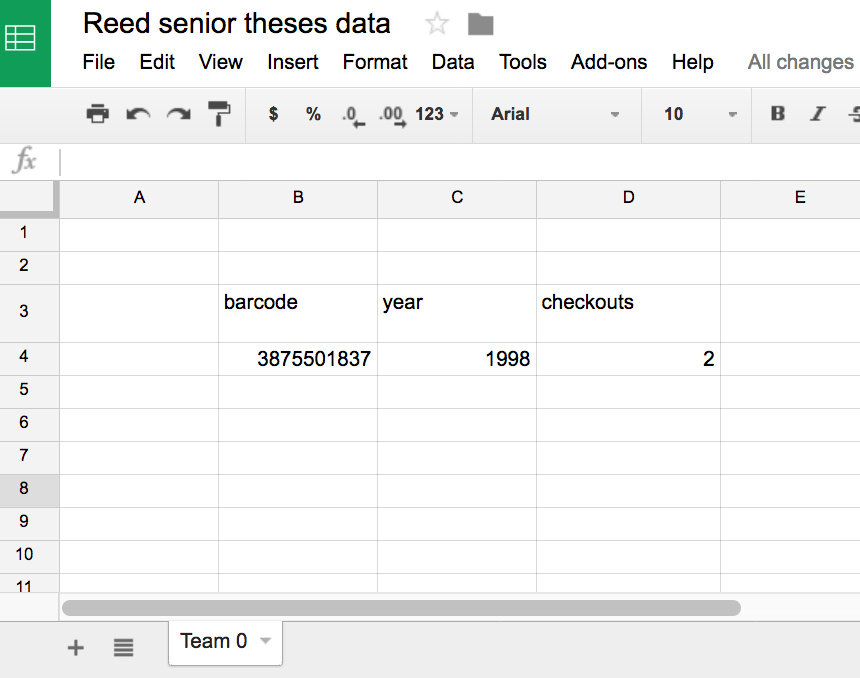
\includegraphics[scale=.5]{senior-thesis-sheets.png}


\end{document}
